\section{Exercise 1 - Mid-depth temperature and \delO{SW} reconstruction}

\begin{figure}
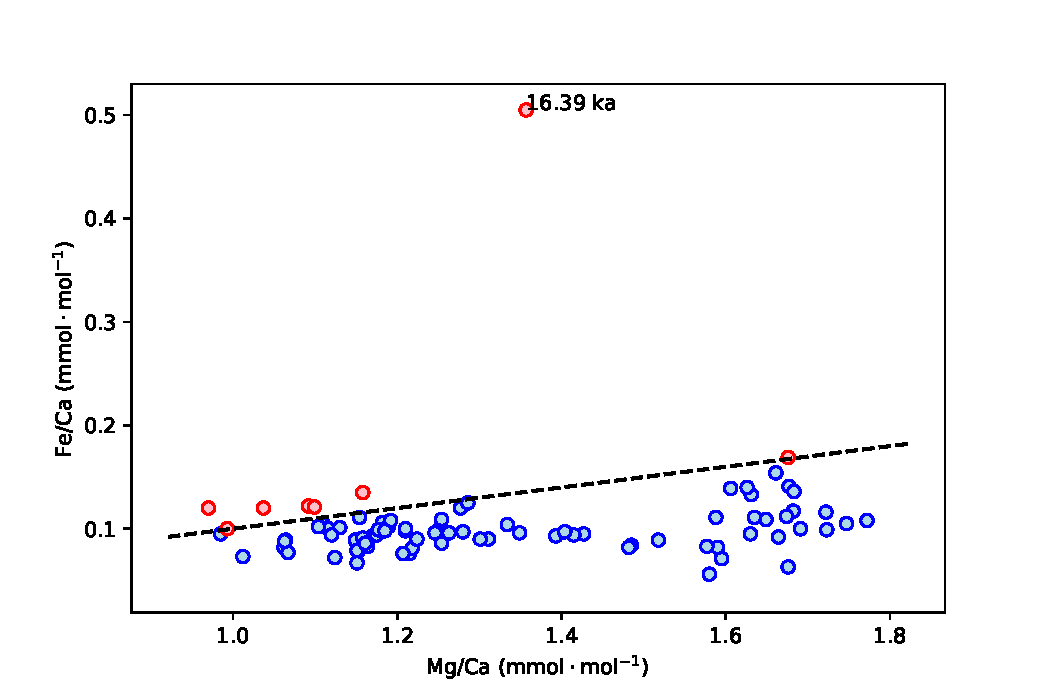
\includegraphics[width=\textwidth]{img/scatter_MgCa_x_FeCa_contaminated.pdf}
    \caption{Scatter plot of bottom water temperature from Mg/Ca palaeothermometry against ice volume corrected oxygen isotope excursion (\delO{SW}), both from benthic foraminifera M. barleeanuum.
             Red points mark potentially contaminated measurements.}
        \label{fig:Mg_Fe}
\end{figure}

\begin{figure}
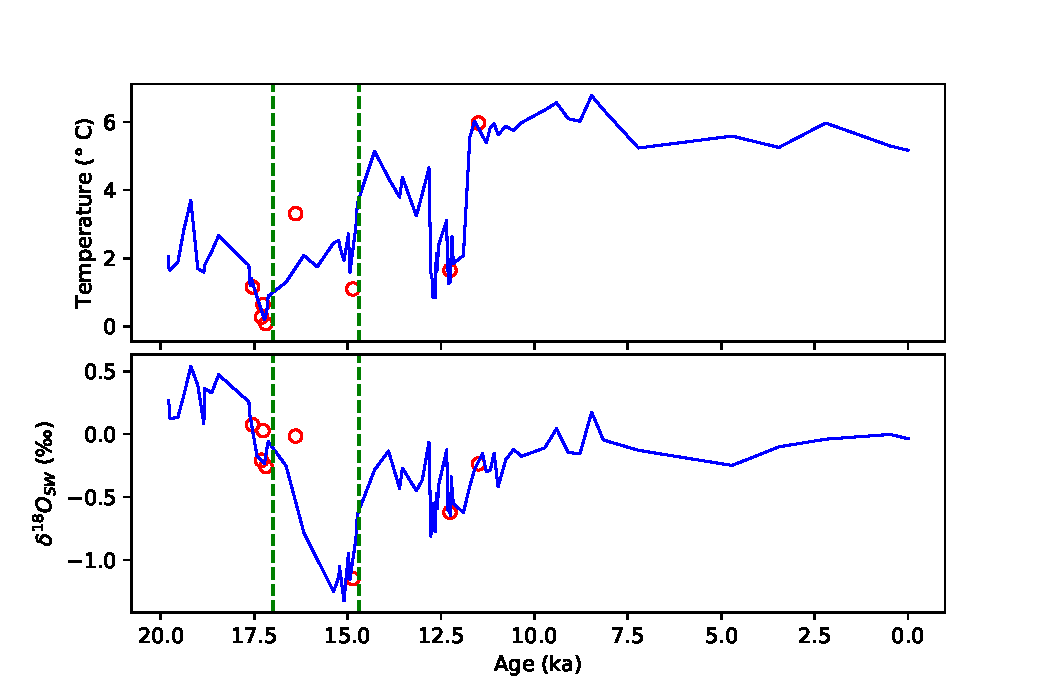
\includegraphics[width=\textwidth]{img/timeseries_temp_and_d18Osw.pdf}
    \caption{Time series of: ice-volume corrected oxygen isotope excursion (top); bottom water temperature (bottom).
             Dashed lines indicate approximate boundaries of Heinrich Stadial 1; red points mark rejected measurements.}
        \label{fig:timeseriestempd18Osw}
\end{figure}

According to \citeauthor{barker2003study}\parencite{barker2003study}, a foramineferal molar ratio of Fe to Mg greater than approximately 0.1 is indicative of potential contamination by clay silicates. Measurements could therefore be rejected by simply applying the criteria:
\begin{equation} \label{eq:fe_mg}
    \frac{\mathrm{Fe}/\mathrm{Ca}}{\mathrm{Mg}/\mathrm{Ca}} > 0.1 \, \mathrm{mol \cdot mol^{-1}}
\end{equation}
However, visual assessment of the magnitude of potential contamination (Figure \ref{fig:Mg_Fe}) shows that, of the 8 measurements meeting the criteria for potential rejection, only one has a Fe/Mg ratio significantly far from the rest of the data. As a result, the 16.39 ka measurement is rejected for contamination. 
